\section{Estrutura da Rede Neural Artificial}

% Equações Governantes
\begin{frame}{Sistema de Compressão e Gás Natural}
    \begin{columns}[T] % [T] alinha as colunas pelo topo
        % Coluna da esquerda - Tabela
        \begin{column}{0.48\textwidth}
        \begin{figure}
            \centering
            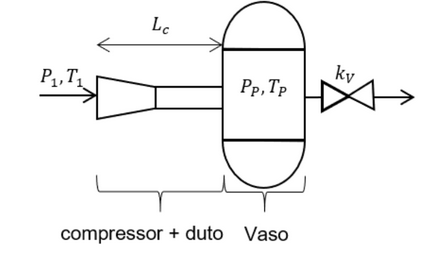
\includegraphics[width=1.1\linewidth]{figures/compressao.png}
            \caption{Sitema de Compressão retirado de Meira et al. (2021)}
            \label{fig:enter-label}
        \end{figure}
        \end{column}

        % Coluna da direita - Composição e EoS
        \begin{column}{0.52\textwidth}
            \scriptsize
        \begin{block}{Composição do gás}
                
            O gás natural utilizado é rico em metano, com composição baseada em Chaczykowski (2009):
            
            \vspace{0.12cm}
            \begin{itemize}  
                \item CH\textsubscript{4}: 98,34\% \quad C\textsubscript{2}H\textsubscript{6}: 0,61\%
                \item C\textsubscript{3}H\textsubscript{8}: 0,15\% \quad iC\textsubscript{4}H\textsubscript{10}: 0,03\%
                \item nC\textsubscript{4}H\textsubscript{10}: 0,03\% \quad CO\textsubscript{2}: 0,80\%
                \item Traços de: iC\textsubscript{5}H\textsubscript{12}, nC\textsubscript{5}H\textsubscript{12}, N\textsubscript{2}
            \end{itemize}
        \end{block}
            \vspace{0.1cm}
            A equação de estado de Soave (1972) foi utilizada para modelar o comportamento termodinâmico do gás:

            \[
            P = \frac{R T}{V - b} - \frac{a(T)}{V(V + b)}
            \]

            com:
            \begin{itemize}
                \item \( a(T) \): fator de correção das forças intermoleculares
                \item \( b \): correção do volume molecular
            \end{itemize}
        \end{column}
    \end{columns}
\end{frame}



\begin{frame}{Equações e Variáveis do Modelo de Meira et al. (2021)}
    \scriptsize
    \textbf{Equações diferenciais que descrevem a dinâmica do sistema:}

    \begin{multicols}{2}
    % Coluna da esquerda: equações
    \begin{align}
        \frac{d\dot{m}}{dt} &= \frac{A_1}{L_c}(P_2 - P_P) \tag{1} \\
        \frac{dV_P}{dt} &= -\frac{V_P^2}{v_{PM}} \left( \dot{m} - \alpha k_v \sqrt{P_P - P_{\text{out}}} \right) \tag{2} \\
        \frac{dT_P}{dt} &= 
        \begin{aligned}[t]
            &\frac{V_P \dot{m}}{v_P M} \left( \frac{h_c - h_p}{C_V} \right) + \\
            + &\frac{R_a T_P}{C_V} \left[ T_P \left( \frac{\partial Z_P}{\partial T} \right)_{V_P} + Z_P \right]
            \frac{V_P}{v_P M} \left( \dot{m} - \alpha k_v \sqrt{P_P - P_{\text{out}}} \right)
        \end{aligned} \tag{3}
    \end{align}

    \columnbreak
    % Coluna da direita: itemize alinhado à direita usando minipage
    \begin{minipage}{\linewidth}
        \raggedleft
        \textbf{Principais variáveis algébricas estimadas:}
        \begin{itemize}
            \item \( P_2 \), \( T_2 \), \( V_2 \): saída do compressor
            \item \( T_{2s} \), \( V_{2s} \): pós-compressão isentrópica
            \item \( V_1 \): sucção do compressor
            \item \( V_{imp} \), \( T_{imp} \): impelidor
            \item \( V_{dif} \), \( T_{dif} \): difusor
            \item \( P_P \): pressão no plenum
        \end{itemize}
    \end{minipage}
    \end{multicols}

    \vspace{0.2cm}
    \textbf{Símbolos:}
    \begin{itemize}
        \item \( \dot{m} \): vazão mássica; 
        \( V_P \), \( T_P \), \( Z_P \): volume molar, temperatura e fator de compressibilidade no plenum;
        \( R_a \): constante dos gases; 
        \( M \): massa molar; 
        \( h_c \), \( h_p \): entalpias; 
        \( C_V \): calor específico a volume constante.
    \end{itemize}
\end{frame}

\begin{frame}{Estrutura da Rede Neural Proposta}
    \vspace{-0.3cm}
    \begin{figure}
        \centering
        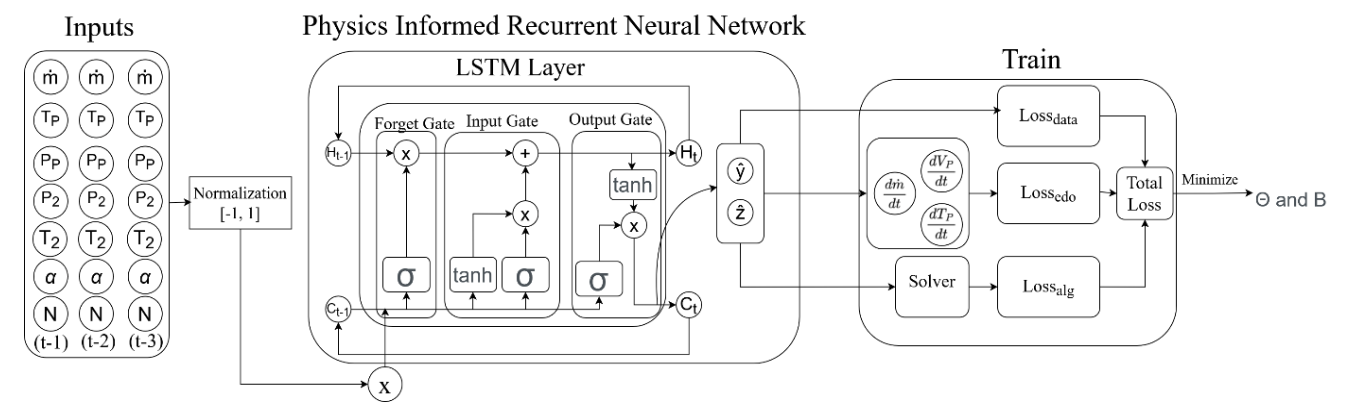
\includegraphics[width=1.0\textwidth]{figures/PIRNN.png} % Insira o caminho correto para a imagem
        \caption{\small Diagrama da arquitetura da PINN.}
    \end{figure}
\end{frame}
\begin{frame}{Função de Loss e Hiperparâmetros da Rede}
    \begin{columns}[T]
        % Coluna da esquerda - Função de perda
        \begin{column}{0.55\textwidth}
            \footnotesize
            A equação geral da função de perda utilizada foi:

            \[
            \text{Loss} = \frac{1}{N} \sum_{i=1}^{N} (\hat{y}_i^* - y_i^*)^2
            + \frac{1}{N} \sum_{i=1}^{N} \left( \frac{d\hat{y}_{i,\text{num}}}{dt} - \frac{d\hat{y}_{i,\text{an}}}{dt} \right)^2
            + \frac{1}{N} \sum_{i=1}^{N} (\hat{z}_i - z_i)^2
            \]

            \vspace{0.2cm}
            Onde:
            \begin{itemize}
                \item \( \hat{y}^* \): variáveis previstas mensuráveis (saída da rede);
                \item \( y^* \): variáveis reais mensuráveis (target);
                \item \( \hat{z} \): variáveis algébricas previstas pela rede;
                \item \( z \): variáveis algébricas calculadas pelo solver extermp.
            \end{itemize}
        \end{column}

        % Coluna da direita - Tabela de hiperparâmetros
        \begin{column}{0.45\textwidth}
            \vspace{2cm}
            \begin{block}{\centering Hiperparâmetros do Modelo}
                \footnotesize
                \centering
                \resizebox{\linewidth}{!}{%
                    \begin{tabular}{p{3.6cm} p{2.4cm}}
                        \toprule
                        \textbf{Parâmetro} & \textbf{Valor} \\
                        \midrule
                        Nº de camadas (LSTM) & 1 \\
                        Learning Rate inicial & $1 \cdot 10^{-4}$ \\
                        Tamanho do mini batch & 64 \\
                        Neurônios por camada & 100 \\
                        Nº de épocas & 200 \\
                        Otimizador & Adam \\
                        \bottomrule
                    \end{tabular}%
                }
            \end{block}
        \end{column}
    \end{columns}
\end{frame}

\begin{frame}{Resultados de Previsão e Erro Quadrático Médio}
\scriptsize

\begin{center}
% Linha de imagens lado a lado
\setlength{\fboxsep}{0pt}% remove espaço extra
\begin{minipage}[t]{0.49\textwidth}
    \centering
    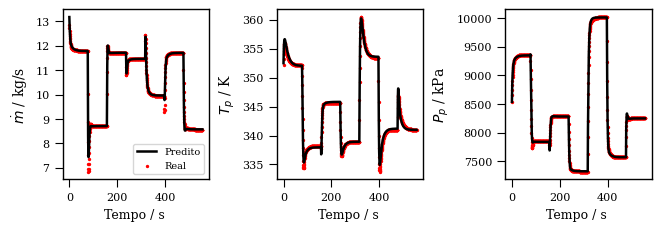
\includegraphics[width=1.05\linewidth, height=0.40\textheight, keepaspectratio]{figures/plot_1.png}
    \vspace{0.1cm}
    {\tiny\parbox{\linewidth}{\centering Comparação entre o modelo de rede neural e os dados simulados para vazão mássica, temperatura no plenum ($T_P$) e pressão no plenum ($P_P$).}}
\end{minipage}\hfill
\begin{minipage}[t]{0.49\textwidth}
    \centering
    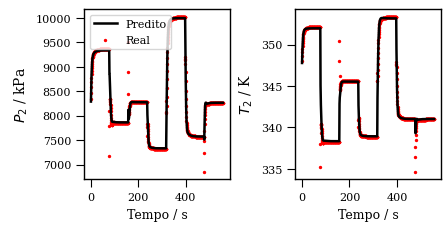
\includegraphics[width=1.1\linewidth, height=0.4\textheight, keepaspectratio]{figures/plot_2.png}
    \vspace{0.1cm}
    {\tiny\parbox{\linewidth}{\centering Comparação entre o modelo de rede neural e os dados simulados para a pressão ($P_2$) e a temperatura ($T_2$) na saída do compressor.}}
\end{minipage}
\end{center}

\vspace{0.2cm}

% Linha da tabela
\centering
\textbf{Raiz do Erro Quadrático Médio (RMSE) das demais variáveis} \\[0.2cm]

\begin{tabular}{@{}ccccccc@{}}
\toprule
$V_P$ & $T_{imp}$ & $V_{imp}$ & $T_{dif}$ & $V_{dif}$ & $T_{2s}$ & $V_{2s}$ \\
\midrule
0.012762 & 0.050806 & 0.045487 & 0.049855 & 0.031096 & 0.037175 & 0.037160 \\
\bottomrule
\end{tabular}

\end{frame}

\begin{frame}{Distribuição do Tempo de Simulação}
\centering
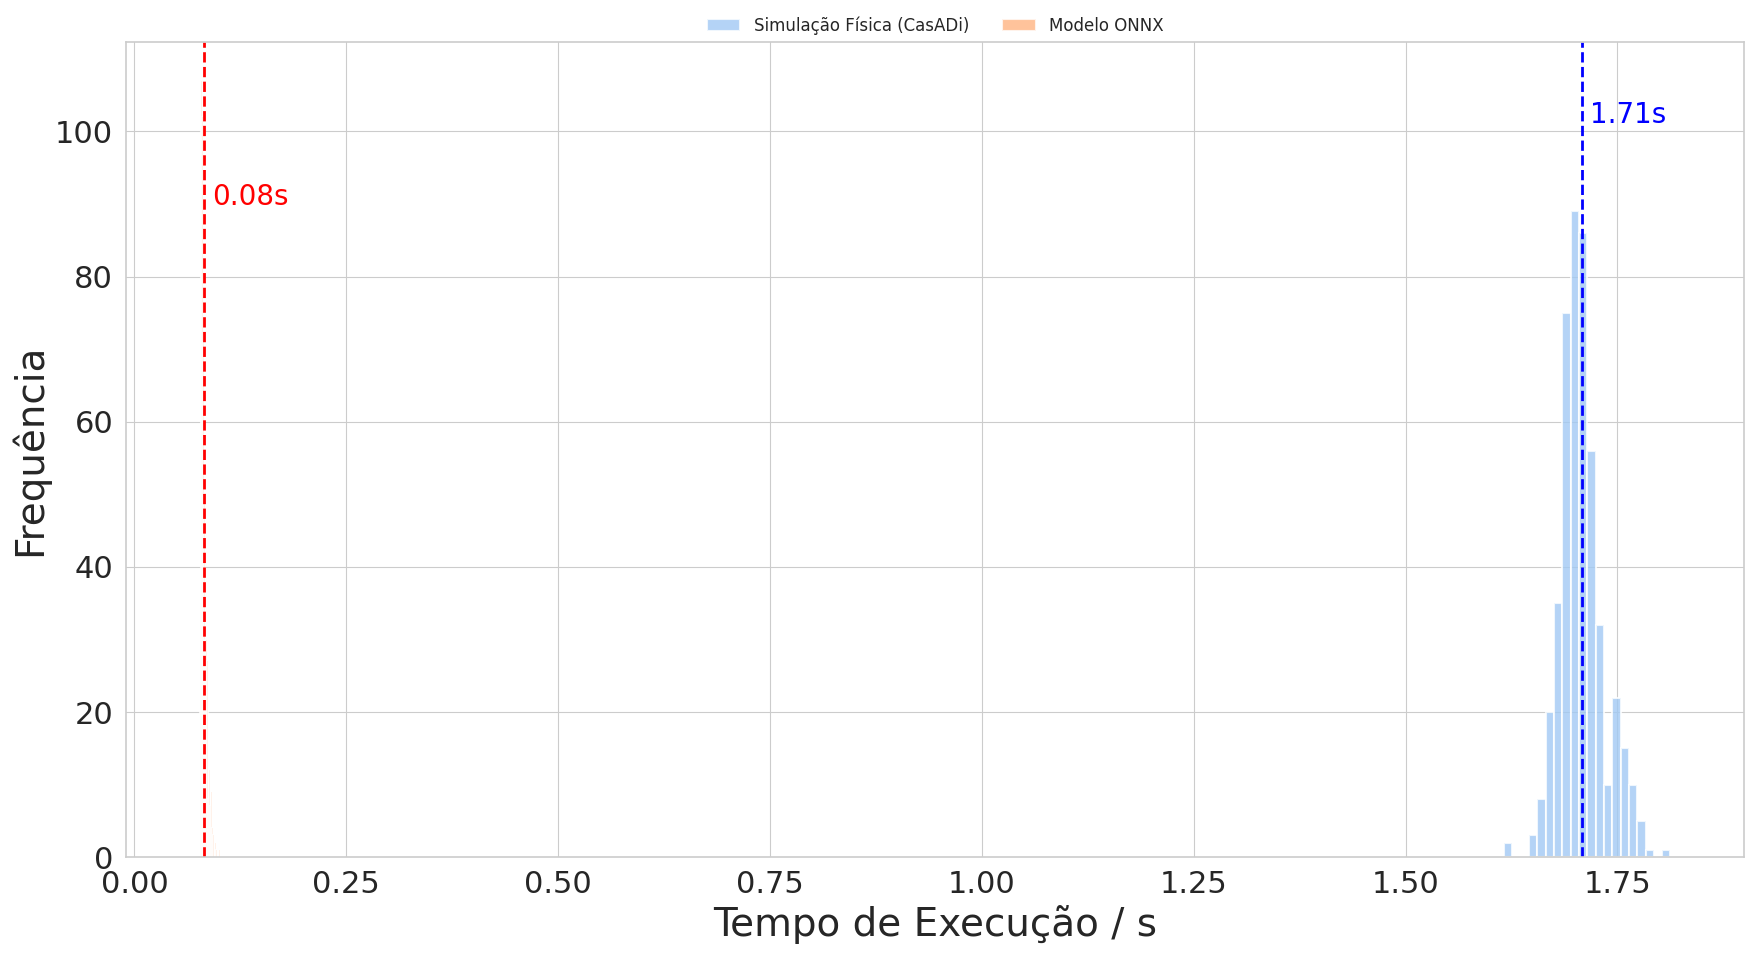
\includegraphics[width=0.8\textwidth]{figures/hist.png}

\vspace{0.3cm}
{\scriptsize Distribuição do tempo de simulação dos experimentos/modelos.}
\end{frame}




